%% these.tex
%% Copyright 2010 Luca De Feo
%% All rights reserved


\section{Arithmetic circuits}
\label{sec:circuits}

\index{arithmetic~circuit}In this section we briefly present the
arithmetic circuit model. Since we have in mind applications to the
theory of transposition, our presentation slightly deviates from
textbooks; for a more classical and extensive treatment see
\cite{burgisser+clausen-shokrollahi,vollmer}.

\subsection{Basic definitions}
In the whole chapter, by $R$ we shall denote a (non necessarily
commutative) ring with unit. Unless otherwise stated, we consider
$R^n$ with its natural structure of left $R$-module; when needed, we
shall use \hyperref[sec:linear-algebra:bra-ket]{kets} $\ket{x}$ to
remove any ambiguity about the fact that we are talking about elements
of a left module.  We set $R^0=0$, the zero module, and we denote by
$\bom$ (or $\ket{\bom}$) its unique element.

The dual space $\dual{(R^n)}=\hom(R^n,R)$ has a natural structure of
right $R$-module (equivalently, of left $R^\op$-module) by the
assignment
\begin{equation}
  \label{eq:232}
  \bra{\ell} a : \ket{x} \mapsto \braket{\ell}{x}a
  \text{,}
\end{equation}
where we have used \hyperref[sec:linear-algebra:bra-ket]{bras} to
denote elements of $\dual{(R^n)}$ and a
\hyperref[sec:linear-algebra:bra-ket]{bracket} to denote the natural
bilinear form that results by applying linear forms to elements.

\begin{definition}[Arithmetic operator, arity]
  An \index{arithmetic~operator}\emph{arithmetic operator} over $R$ is
  a morphism of left modules $f:R^i\ra R^o$ for some $i,o\in\N$. Here
  $i$ is called the \index{arity}\emph{in-arity} of $f$ or simply
  \emph{arity}, $o$ is called the \emph{out-arity} of $f$.
\end{definition}

\begin{definition}[Arithmetic basis]
  An \index{arithmetic~basis}\emph{arithmetic $R$-basis} is a (not
  necessarily finite) set of arithmetic operators over $R$.  A basis
  is said to be \index{arithmetic~basis!commutative}\emph{commutative}
  if all its operators are invariant under the natural action of
  $\mathcal{S}_n$ over $R^n$ (i.e.\ under permutation of coordinates).
\end{definition}

\pdfmctwo{Added parentheses in the definition of the bases,
  hope it helps reading.}  The arithmetic basis we will work with is
the \index{standard~left-linear~basis}\emph{standard left-linear
  basis}, denoted by $\Tbasis$.  It is composed of
\begin{equation}
  \label{eq:tbasis}
  \tag{$\Tbasis$}
  \begin{aligned}
    + : R\oplus R &\ra R\text{,}    & \rmul{a} : R &\ra R\text{,}     &  \hub : R &\ra R\oplus R\text{,}\\
      (a, b) &\mapsto a+b\text{,}   &           b &\mapsto ba\text{,} &         a &\mapsto (a,a)\text{,}\\ \\
    0 : 0 &\ra R\text{,}     &&& \omega : R &\ra 0\text{,} \\
     \bom &\mapsto 0\text{,} &&&          a &\mapsto \bom\text{.}
  \end{aligned}
\end{equation}
Arithmetic circuits are directed acyclic multigraphs carrying
information from an arithmetic basis; the formal definition follows.

\begin{definition}[Arithmetic node]
  Let $\mathcal{B}$ be an $R$-basis. A \index{node}\emph{node} over
  $(R,\mathcal{B})$ is a tuple $v=(I, O, f)$ such that
  \begin{itemize}
  \item $I$ and $O$ are finite ordered sets, 
  \item $f$ is either an element of $\mathcal{B}$ or the special value
    $\emptyset$.
  \item If $f=\emptyset$, one of the two following conditions must hold:
    \begin{itemize}
    \item $I$ is a singleton and $O$ is empty, in this case we say
      that $v$ is an \index{node!input~node}\emph{input node};
    \item $I$ is empty and $O$ is a singleton, in this case we say
      that $v$ is an \index{node!output~node}\emph{output node}.
    \end{itemize}
  \item If $f\ne\emptyset$, the cardinality of $I$ matches the
    in-arity of $f$ and the cardinality of $O$ matches the out-arity
    of $f$; in this case we say that $v$ is an
    \index{node!evaluation~node}\emph{evaluation node}.
  \end{itemize}
\end{definition}

\begin{figure}[!ht]
  \label{fig:nodes}
  \centering
  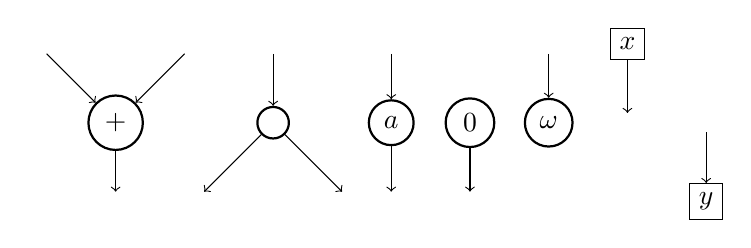
\begin{tikzpicture}
    \tikzstyle{node}=[circle,thick,draw=black,minimum size=4mm]
    \tikzstyle{arg}=[rectangle,thin,draw=black,minimum size=4mm]
    
    \begin{scope}
      \node(in1){};
      \node(nop)[right of=in1]{};
      \node(in2)[right of=nop]{};

      \node[node](plus)[below of=nop]{$+$};
      \node(out)[below of=plus]{};

      \path[->]
      (in1) edge (plus)
      (in2) edge (plus)
      (plus) edge (out);
    \end{scope}
    
    \begin{scope}[xshift=30mm]
      \node(in){};
      \node[node](hub)[below of=in]{$\hub$};
      \node(nop)[below of=hub]{};
      \node(out1)[left of=nop]{};
      \node(out2)[right of=nop]{};

      \path[->]
      (in) edge (hub)
      (hub) edge (out1)
      (hub) edge (out2);
    \end{scope}
    
    \begin{scope}[xshift=45mm]
      \node(in){};
      \node[node](times)[below of=in]{$\rmul{a}$};
      \node(out)[below of=times]{};

      \path[->]
      (in) edge (times)
      (times) edge (out);
    \end{scope}

    \begin{scope}[xshift=55mm]
      \node(nop){};
      \node[node][below of=nop](create){$0$};
      \node(out)[below of=create]{};
      \path[->] (create) edge (out);
    \end{scope}

    \begin{scope}[xshift=65mm]
      \node(in){};
      \node[node][below of=in](destroy){$\omega$};
      \node(nop)[below of=destroy]{};
      \path[->] (in) edge (destroy);
    \end{scope}

    \begin{scope}[xshift=75mm]
      \node[arg](in){$x$};
      \node[below of=in](out){};
      \path[->] (in) edge (out);
    \end{scope}

    \begin{scope}[xshift=85mm]
      \node(nop){};
      \node[below of=nop](in){};
      \node[arg](out)[below of=in]{$y$};
      \path[->] (in) edge (out);
    \end{scope}
  \end{tikzpicture}
  \caption{Nodes over the standard linear basis: round ones are
    evaluation nodes, square ones are input and output nodes.}
\end{figure}


We call \index{port!input~port}\emph{input ports} the elements of $I$
and \index{port!output~port}\emph{output ports} the elements of $O$,
which we denote respectively by
$\inp(v)$\symb[port-in]{$\inp(v)$}{Input ports of a node} and
$\outp(v)$\symb[port-out]{$\outp(v)$}{Output ports of a
  node}. The cardinalities of $I$ and $O$ are called, respectively,
the \index{node!degree}\emph{in-degree} and \emph{out-degree} of $v$.
We call $f$ the \index{node!value}\emph{value} of $v$ and write
$\beta(v)$ for it.

Nodes over the linear basis are pictured in Figure~\ref{fig:nodes}. We
do not explicitly represent the orderings on $\inp(+)$ and
$\outp(\hub)$ because they are not relevant for the linear basis: in
fact, all operators are commutative.

\begin{definition}[Arithmetic circuit]
  Let $\mathcal{B}$ be an $R$-basis. A (linear)
  \index{arithmetic~circuit}\emph{arithmetic circuit} over
  $(R,\mathcal{B})$ is a tuple $C=(V,E,\le,\le_i,\le_o)$ such that
  \begin{enumerate}
  \item $V$ is a finite set of nodes over $(R,\mathcal{B})$;
  \item $<$ is a total order on $V$, $<_i$ is a total order on the
    input nodes in $V$, $<_o$ is a total order on the output nodes in
    $V$;
  \item let $I=\biguplus_{v\in V}\inp(v)$ and $O=\biguplus_{v\in
      V}\outp(v)$, then $E$ is a bijection from $O$ to $I$ such that
    $E(o)=i$ implies that $o\in\outp(v)$, $i\in\inp(v')$ and $v\lneq
    v'$.
  \end{enumerate}
\end{definition}

In practice, the definition says that $C$ is a directed acyclic
multigraph (also called \index{multiDAG}\emph{multiDAG}), where $V$
are the \index{vertex}vertices, $E$ the \index{edge}edges, and where
the \index{node!degree}degrees of each vertex are prescribed by the
arities of the underlying arithmetic node. Moreover, we add an
ordering on input nodes (vertices of in-degree $0$) and on output
nodes (vertices of out-degree $0$). 

In what follows, we shall call $(V,E)$ the
\index{underlying~graph}\emph{underlying graph} of $C$, and use
classic graph theoretic terms to refer to its properties. We shall
often implicitly make this identification. Thus, we shall represent
$E$ as a set of edges $(o,i)$, and make use of the classic concepts of
\emph{incident} edge, nodes \emph{connected} by an edge,
\index{path}\emph{paths}, etc.

Figure~\ref{fig:circuit} shows two examples of arithmetic circuits.
Input and output nodes are ordered from left to right; ports are not
ordered because the basis is commutative.


\begin{figure}[!ht] \centering
  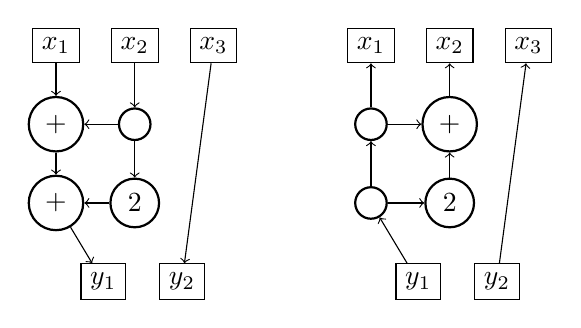
\begin{tikzpicture}
\tikzstyle{node}=[circle,thick,draw=black,minimum size=4mm]
\tikzstyle{arg}=[rectangle,thin,draw=black,minimum size=4mm]
    
    \begin{scope} \node[arg](in1){$x_1$}; \node[arg,right
of=in1](in2){$x_2$}; \node[arg,right of=in2](in3){$x_3$};
      
      \node[node,below of=in1](plus1){$+$}; \node[node,right
of=plus1](H){$\hub$};

      \node[node,below of=plus1](plus2){$+$}; \node[node,right
of=plus2](times){$\rmul{2}$};

      \node[arg,below of=plus2,xshift=6mm](out1){$y_1$};
\node[arg,right of=out1](out2){$y_2$};

      \path[->] (in1) edge (plus1) (in2) edge (H) (in3) edge (out2)
(H) edge (plus1) (H) edge (times) (plus1) edge (plus2) (times) edge
(plus2) (plus2) edge (out1);
    \end{scope}

    \begin{scope}[xshift=4cm]
      \node[arg](in1){$\dual{x_1}$};
      \node[arg,right of=in1](in2){$\dual{x_2}$};
      \node[arg,right of=in2](in3){$\dual{x_3}$};
      
      \node[node,below of=in1](plus1){$\hub$};
      \node[node,right of=plus1](H){$+$};

      \node[node,below of=plus1](plus2){$\hub$};
      \node[node,right of=plus2](times){$\rmul{2}$};

      \node[arg,below of=plus2,xshift=6mm](out1){$\dual{y_1}$};
      \node[arg,right of=out1](out2){$\dual{y_2}$};

      \path[<-]
      (in1) edge (plus1)
      (in2) edge (H)
      (in3) edge (out2)
      (H) edge (plus1)
      (H) edge (times) 
      (plus1) edge (plus2)
      (times) edge (plus2)
      (plus2) edge (out1);
    \end{scope}
  \end{tikzpicture}
  \caption{Two arithmetic circuits over $\Tbasis$. The linear map
    $y_1=x_1+3x_2, y_2=x_3$ is computed by the circuit on the left and
    its dual is computed by the circuit on the right.}
  \label{fig:circuit}
\end{figure}

\begin{definition}[Size, depth]
  \label{def:size}
  Let $C$ be a circuit over $(R,\mathcal{B})$. The
  \index{arithmetic~circuit!size}\emph{size} of $C$, denoted by
  $\size(C)$\symb[circuit-size]{$\size_X(C)$}{Size
    ($X$-weighted) of an arithmetic circuit} is the number of
  evaluation nodes in $V$; the
  \index{arithmetic~circuit!depth}\emph{depth} of $C$, denoted by
  $\depth(C)$\symb[circuit-depth]{$\depth(C)$}{Depth of an
    arithmetic circuit} is the length of the longest directed path
  --in a graph-theoretic sense-- in $(V,E)$.

  Sometimes it is useful to only count certain nodes. Let
  $X\subset\mathcal{B}$, the
  \index{arithmetic~circuit!weighted~size}$X$-weighted size of $C$,
  denoted by $\size_X(C)$ is the number of nodes $v\in V$ such that
  $\beta(v)\in X$.
\end{definition}


\subsection{Semantic of a circuit}
\label{sec:semantic-circuit}
Circuits would be meaningless if they had no semantic attached to
them. Intuitively the semantic corresponds to recursively feed inputs
to the nodes, evaluate $\beta(v)$ at the inputs and collect the
outputs.

\begin{definition}[Evaluation of an arithmetic circuit]
  \label{def:eval}
  \index{arithmetic~circuit!semantic}\index{arithmetic~circuit!evaluation}
  Let $C$ be an arithmetic circuit with $i$ inputs and $o$ outputs,
  then its evaluation is a morphism $\eval_C:R^i\ra
  R^o$\symb[eval]{$\eval_C$}{Evaluation of an arithmetic
    circuit}.

  In order to define it, we simultaneously define the evaluation
  $\eval_v$ of each $v\in V$ and the evaluation $\eval_e$ of each
  $e\in E$. We will denote by $<_v$ the orders on the input and the
  output ports of $v$.
  \begin{itemize}
  \item Let $v\in V$ have out-degree $n$, let its evaluation be
    $\eval_v:R^i\ra R^n$ and let $\pi_1,\ldots,\pi_n$ be the canonical
    projections from $R^n$ to $R$. Let $o_1<_v\cdots<_vo_n$ be the
    output ports of $v$ and let $e_j=\bigl(o_j,E(o_j)\bigr)$ be the
    corresponding edges stemming from $v$, then $\eval_{e_j} =
    \pi_j\circ\eval_v$ for any $j$.
  \item Let $x_1<_i\cdots<_ix_i$ be the input nodes and let
    $\pi_1,\ldots,\pi_i$ be the canonical projections from $R^i$ to
    $R$, then $\eval_{x_j}=\pi_j$ for any $j$.
  \item For every evaluation node $v$ with in-degree $m$, let
    $i_1<_v\cdots<_vi_m$ be the input ports of $v$ and let
    $e_j=\bigl(E^{-1}(i_j),i_j\bigr)$ be the corresponding edges
    incident to $v$, then
    \begin{equation}
      \label{eq:eval_v}
      \eval_v = \beta(v) \circ (\eval_{e_1}, \cdots,\eval_{e_m})
      \text{.}
    \end{equation}
  \item For every output node $y$, let $e\in E$ be the only edge
    incident to $y$, then $\eval_y=\eval_e$.
  \end{itemize}

  We can finally define $\eval_C:R^i\ra R^o$. Let $y_1<_o\cdots<_oy_o$
  be the output nodes, then
  \begin{equation}
    \label{eq:eval}
    \eval_C = \left(\eval_{y_1}, \cdots,\eval_{y_o}\right)
    \text{.}
  \end{equation}
  We also say that $C$ \emph{computes} $\eval_C$.
\end{definition}

It is immediate to verify that $\eval_C$ is a morphism of left
modules, because we only used compositions and direct sums to define
it. The converse is partially true.

\begin{proposition}
  Any morphism of free finite-dimensional $R$-modules can be computed
  by an arithmetic circuit over $(R,\Tbasis)$.
\end{proposition}
\begin{proof}
  Take the matrix associated to such morphism and create a circuit
  that performs the matrix-vector product.
\end{proof}

This also gives an upper bound of $O(mn)$ on the circuit size of a
linear operator $R^m\ra R^n$.

We now define a way of substituting nodes, first syntactically, then
semantically.

\begin{definition}[Syntactic substitution]
  \label{def:syntax-subst}\index{arithmetic~circuit!substitution}
  Let $C=(V,E,\le,\le_i,\le_o)$ be a circuit over $(R,\mathcal{B})$
  and let $C'=(V',E',\le',\le_i',\le_o')$ be a circuit over
  $(R,\mathcal{B}')$. Let $C'$ have $i$ inputs and $o$ outputs and let
  $v\in V$ have in-degree $i$ and out-degree $o$.

  Let $\mathcal{I}$ and $\mathcal{O}$ be monotone bijections
  respectively from $\inp(v)$ to $\inp(C')$ and from $\outp(C')$ to
  $\outp(v)$. We denote by $C[C'/v]$ the circuit
  $(V'',E'',\le'',\le_i'',\le_o'')$ over
  $(R,\mathcal{B}\cup\mathcal{B}')$ defined as follows:
  \begin{itemize}
  \item $V'' = V\uplus (V' - \inp(C') - \outp(C'))$;
  \item $\le_i''=\le_i$, $\le_o''=\le_o$;
  \item $v'\le v''$ if and only if one of the following conditions hold:
    \begin{itemize}
    \item $v',v''\in V$ and $v'\le v''$;
    \item $v',v''\in V'$ and $v'\le' v''$;
    \item $v'\in V$ and $v''\in V'$ and $v'\le v$;
    \item $v'\in V'$ and $v''\in V$ and $v\le v''$;
    \end{itemize}
  \item $E''(o) = \begin{cases}
      E'(o') & \text{if $E(o)\in\inp(v)$ and $\mathcal{I}(E(o))=v'$ and $\outp(v')=\{o'\}$,}\\
      E(o') & \text{if $E'(o)\in\outp(C')$ and $\mathcal{O}(E'(o))=o'$,}\\
      (E\uplus E')(o) & \text{otherwise.}
    \end{cases}$
  \end{itemize}
\end{definition}

\begin{definition}[Semantic substitution]
  \label{def:sem-subst}\index{arithmetic~circuit!substitution}
  Let $C$ be a circuit over $(R,\mathcal{B}\cup\{f\})$ and let $F$ be
  a circuit over $(R,\mathcal{B})$ such that $\eval_F=f$.

  We denote by $C[F/f]$ the circuit over $(R,\mathcal{B})$ where any
  node $v$ of $C$ such that $\beta(v)=f$ has been syntactically
  substituted by $F$.
\end{definition}

The proof of the following proposition is immediate.

\begin{proposition}
  Under the conditions of the previous definition,
  \[\eval_{C[F/f]} = \eval_C \text{.}\]
\end{proposition}

As a shorthand notation, we will draw octogones to signify that a node
has been syntactically substituted by a circuit, without giving the
actual shape of the substituting circuit. Figure
\ref{fig:substitution} shows an example.

\begin{figure}[!ht]
  \label{fig:substitution}
  \centering
  \begin{tikzpicture}
    \tikzstyle{node}=[circle,thick,draw=black,minimum size=4mm]
    \tikzstyle{arg}=[rectangle,thin,draw=black,minimum size=4mm]
    \tikzstyle{subst}=[regular polygon,regular polygon sides=8,thick,draw=black,minimum size=4mm]
    
    \begin{scope}
      \node[arg](in1){$x_1$};
      \node[arg,right of=in1](in2){$x_2$};
      
      \node[node](H)[below of=in2]{$\hub$};
      \node[subst](F)[left of=H]{$F$};

      \node[arg,below of=F,xshift=-6mm](out1){$y_1$};
      \node[arg,right of=out1](out2){$y_2$};
      \node[arg,right of=out2](out3){$y_3$};

      \path[->]
      (in1) edge (F)
      (in2) edge (H)
      (H) edge[bend left=10] (F)
      (H) edge[bend right=10] (F)
      (F) edge (out1)
      (F) edge (out2)
      (F) edge (out3);
    \end{scope}

  \end{tikzpicture}
  \caption{Arithmetic circuit where a node has been syntactically
    substituted by a circuit $F$ with $3$ inputs and $3$ outputs.}
\end{figure}



\subsection{The transposition theorem}
\label{sec:tellegen}
We are now ready to state and prove the
\index{transposition~theorem}\emph{transposition theorem} for
arithmetic circuits. 

We fix a family $(M_i)_{i\in\N}$ of free left $R$-modules, with
$M_i\isom R^i$. Via the isomorphisms, it is straightforward to extend
the definition of arithmetic circuit so that $\eval_c$ is a morphism
$M_i\ra M_o$.  We also fix a family $(N_i)_{i\in\N}$ of free right
$R$-modules, and a family of non-degenerate bilinear forms
\begin{equation}
  \label{eq:240}
  \left(\braket{}{}_i:N_i\times M_i\ra R\right)_{i\in\N}
  \text{.}
\end{equation}
One can think of $M_n$ being $R^n$, $N_n$ being $\dual{(R^n)}$, and
the bilinear forms being the natural ones.

We define the notion of dual circuit, that intuitively corresponds to
\emph{turn all the arrows around}.

\begin{definition}[Dual arithmetic basis]
  Let $\mathcal{B}$ be an arithmetic basis over $R$. The
  \index{dual~arithmetic~basis}\emph{dual basis} $\dual{\mathcal{B}}$
  (with respect to $\braket{}{}_i$) is the basis over $R^\op$
  \begin{equation}
    \label{eq:241}
    \dual{\mathcal{B}} = \{\dual{f} \,|\, f\in\mathcal{B}\}
    \text{.}
  \end{equation}
\end{definition}

In particular, the dual basis to $(R,\Tbasis)$ is 
\begin{equation}
  \label{eq:tbasis-star}
  \tag{$\dual{\Tbasis}$}
  \begin{gathered}
    \begin{aligned}
      +=\dual{\hub} : \dual{(R\oplus R)} &\ra \dual{R}\text{,}  &  \hub=\dual{+} : \dual{R} &\ra \dual{(R\oplus R)}\text{,}\\
      \bra{a,b} &\mapsto \bra{a}+\bra{b}\text{,}\qquad   &      \bra{a} &\mapsto \bra{a,a}\text{,}\\
    \end{aligned}\\ \\
    \begin{aligned}
      \rmul{a}=\dual{(\rmul{a})} : \dual{R} &\ra \dual{R}\text{,} \\
                                             \bra{b} &\mapsto \bra{b}a\text{,}
    \end{aligned}\\ \\
    \begin{aligned}
      0=\dual{\omega} : \dual{0} &\ra \dual{R}\text{,}\qquad  & \omega=\dual{0} : \dual{R} &\ra \dual{0}\text{,} \\
      \bra{\bom} &\mapsto \bra{0}\text{,} &          \bra{a} &\mapsto \bra{\bom}\text{.}
    \end{aligned}
  \end{gathered}
\end{equation}

\begin{definition}[Dual circuit]
  \label{def:dual}\index{arithmetic~circuit!dual}
  Let $C=(V,E,\le,\le_i,\le_o)$ be a circuit over
  $(R,\mathcal{B})$. For any $v\in V$ define
  \begin{equation}
    \label{eq:244}
    \dual{v} =
    \begin{cases}
    (O,I,\dual{f})          &\text{if $v=(I,O,f)$ with $f\ne\emptyset$,}\\
    (O,\emptyset,\emptyset) &\text{if $v=(\emptyset,O,\emptyset)$,}\\
    (\emptyset,I,\emptyset) &\text{if $v=(I,\emptyset,\emptyset)$.}
    \end{cases}
  \end{equation}

  The dual circuit (with respect to $\braket{}{}_i$) of $C$, denoted
  by $\dual{C}$, is the arithmetic circuit over
  $(R^\op,\dual{\mathcal{B}})$
  \[\dual{C} = (\dual{V}, E^{-1},\le',\le_i',\le_o')\text{,}\]
  where $\dual{V}=\{\dual{v}|v\in V\}$ and the orderings are defined
  as follows:
  \begin{align}
    v \le v' \;&\Leftrightarrow\; \dual{v'} \le' \dual{v}\text{,}\\
    v \le_o v' \;&\Leftrightarrow\; \dual{v} \le_o' \dual{v'}\text{,}\\
    v \le_i v' \;&\Leftrightarrow\; \dual{v} \le_i' \dual{v'}\text{.}
  \end{align}
\end{definition}

In particular, this makes $(\dual{V},E^{-1})$ the reverse graph of
$(V,E)$ in a graph-theoretic sense. Figure \ref{fig:circuit} shows two
circuits that are each other's dual. We can now state the
transposition theorem.

\begin{theorem}[Transposition theorem]
  \label{th:tellegen}\index{transposition~theorem}
  Let $C$ be a circuit that computes a morphism $f$, then $\dual{C}$
  computes the dual morphism $\dual{f}$.
\end{theorem}

\pdfmctwo{I explain why I postponed the "elegant" proof.}  In order to
maintain this chapter at the level of elementary linear algebra, we
give here a quite tedious proof: it amounts, in a hidden way, to write
down the matrices of $f$ and $\dual{f}$ and check that they are the
same. In Appendix~\ref{cha:basic-categ-theory} we will give a
conceptually simpler proof, using category theory.

\begin{definition}[Evaluation of a path]
  \index{path!evaluation}
  Let $x$ and $y$ be nodes of $C$ and let $p=(e_1,\ldots,e_k)$ be a
  path from $x$ to $y$.

  If $k=1$, we define $\eval_p$ as the identity map $R\ra R$. If
  $k>1$, for any $1\le i<k$ let the node
  \[\xymatrix{\cdots\ar[r]^{e_i}&v\ar[r]^{e_{i+1}}&\cdots}\]
  have $n_i$ inputs and $m_i$ outputs, and let $\iota:R\ra R^{n_i}$ be
  the injection corresponding to the position of $e_i$ in $\inp(v)$
  and $\pi:R^{m_i}\ra R$ the projection corresponding to the position
  of $e_{i+1}$ in $\outp(v)$, then we define
  \begin{equation}
    \label{eq:252}
    f_i = \pi\circ\beta(v)\circ\iota
    \text{.}
  \end{equation}

  Finally, we define $\eval_p$ as
  \begin{equation}
    \label{eq:247}
    f_{k-1}\circ\cdots\circ f_1
    \text{.}
  \end{equation}
\end{definition}

\begin{lemma}[The electrical network lemma]
  \label{th:electrical-network}
  \index{electrical~network~lemma}
  Let $C$ be an arithmetic circuit, let $x_1\le_i\cdots\le_ix_n$ be
  its input nodes and $y_1\le_o\cdots\le_oy_m$ its output nodes. 
  We have the following identity
  \begin{equation}
    \label{eq:248}
    \pi_j\circ\eval_C\circ\iota_i =
    \sum_{p\in x_i\leadsto y_j}\eval_p
    \quad\text{for any $1\le i\le n$, $1\le j\le m$,}
  \end{equation}
  where the sum ranges over all the distinct paths from $x_i$ to
  $y_j$.
\end{lemma}
\begin{proof}
  \pdfmctwo{Patched proof, finally it is correct!}
  We start by proving that for any node $v$ and any edge
  $v\overset{e}{\ra}v'$
  \begin{equation}
    \label{eq:250}
    \eval_{e} = \sum_{i=1}^n\sum_{p\in x_i\leadsto v\overset{e}{\ra}v'}\eval_p\circ\pi_i
    \text{,}
  \end{equation}
  where $\pi_i:R^n\ra R$ is the $i$-th projection, and the second sum
  ranges over all the distinct paths from $x_i$ to $v'$ passing
  through $e$. We do this by induction on the length of the longest
  path to $v$.

  If the longest path to $v$ has length $0$, then $v$ is one of the
  input nodes, say $x_i$. Then by \hyperref[def:eval]{definition}
  $\eval_e=\pi_i$, and Eq.~\eqref{eq:250} is verified.

  Then, let $v$ be an evaluation node, let $e_1\le_v\ldots\le_ve_k$ be
  the edges incident to $v$, and let $v_1,\ldots,v_k$ be the
  corresponding nodes. Then, by \hyperref[def:eval]{definition}
  \begin{equation}
    \label{eq:251}
    \eval_{e} = \pi_e\circ\beta(v)\circ(\eval_{e_1},\ldots,\eval_{e_k}) =
    \sum_{j=1}^k \pi_e\circ\beta(v)\circ\iota_j\circ\eval_{e_j}
    \text{,}
  \end{equation}
  where $\pi_e$ is the projection corresponding to the position of $e$
  in $\outp(v)$. By induction, this is equivalent to
  \begin{equation}
    \label{eq:253}
    \sum_{j=1}^k\sum_{i=1}^n\sum_{p\in x_i\leadsto v_j\overset{e_j}{\ra}v} \pi_e\circ\beta(v)\circ\iota_j\circ\eval_p\circ\pi_i =
    \sum_{i=1}^n\sum_{p\in x_i\leadsto v\overset{e}{\ra}v'}\eval_p\circ\pi_i
    \text{,}
  \end{equation}
  where the equality comes from Eq.~\eqref{eq:252}.

  Now, by the \hyperref[def:eval]{definition} of $\eval_C$ we have
  \begin{equation}
    \label{eq:254}
    \pi_j\circ\eval_C = \eval_{y_j} = \sum_{i=1}\sum_{p\in x_i\leadsto y_j}\eval_p\circ\pi_i
    \text{,}
  \end{equation}
  and composing on both sides with $\iota_i$ gives Eq.~\eqref{eq:248}.
\end{proof}


\begin{proof}[Proof of the transposition theorem]
  The proof of the transposition theorem is now straightforward. By linearity
  it is enough to prove that
  \begin{equation}
    \label{eq:242}
    \pi_j\circ\eval_C\circ\iota_i =
    \dual{\left(\pi_i\circ\eval_{\dual{C}}\circ\iota_j \right)}
    \quad\text{for any $1\le i\le n$, $1\le j\le m$,}
  \end{equation}
  but this is evident by Eqs.~\eqref{eq:248},~\eqref{eq:247}
  and~\eqref{eq:252}.
\end{proof}

\begin{corollary}
  \label{th:tellegen-coro}
  A linear function $f:R^n\ra R^m$ and its transpose can be computed
  by arithmetic circuits on $(R,\Tbasis)$ of same sizes and depths. In
  particular if $C$ computes $f$ and $\dual{C}$ computes $\dual{f}$,
  \begin{gather*}
    \size_{\{+\}}(C) = \size_{\{\hub\}}(\dual{C}), \qquad  
    \size_{\{\hub\}}(C) = \size_{\{+\}}(\dual{C}), \\
    \size_{\{*_a\}}(C) = \size_{\{*_a\}}(\dual{C})\quad\text{for any $a\in R$},\\
    \size_{\{0\}}(C) = \size_{\{\omega\}}(\dual{C}), \qquad 
    \size_{\{\omega\}}(C) = \size_{\{0\}}(\dual{C}).
  \end{gather*}
\end{corollary}

\begin{remark}
  \label{rk:tellegen}
  The name ``transposition theorem'' is somehow misleading. In fact,
  the theorem says that if $\eval_C$ is the map $x\mapsto xM$ for some
  matrix $M$, then $\eval_{\dual{C}}$ is the map $y\mapsto My$. If $R$
  is commutative, this is equivalent to transpose $M$, but in the
  non-commutative case this is not true anymore. For this reason, we
  shall always prefer the formulation in terms of bilinear forms
  instead of the one in terms of matrices.

  \pdfmcone{Dropped comment about quantum computing: it is
    more complicated than that (and I did not want to develop it in the
    appendix).}  It is also worth noticing that the transposition
  theorem stays true if instead of a bilinear form we had used a
  sesquilinear form (in this case $\dual{(\rmul{a})}=\rmul{\bar{a}}$).
\end{remark}


\begin{nota}
  The name ``The electrical network lemma'' is ours, but it could well
  have been original. The transposition theorem was first discovered
  in electrical network theory by Bordewijk~\cite{bordewijk57}; he
  only showed the case $R=\C$. Some attribute the discovery to
  Tellegen~\cite{burgisser+clausen-shokrollahi,bostan+lecerf+schost:tellegen},
  Bordweijk's advisor, but this is debated~\cite{djb:tellegen}.

  The first complete algebraic proof, treating the case of an
  arbitrary non-commutative ring, is due to
  Fiduccia~\cite{fiduccia:phd}. There have been many rediscoveries of
  the theorem (see~\cite{djb:tellegen}), but Fiduccia's statement stays
  the most general.

  Canny, Kaltofen and Yagati~\cite{canny+kaltofen+yagati89,Ka2K}
  pointed out that the transposition theorem can be proven as a
  special case of Baur and Strassen's differentiation of
  circuits~\cite{baur+strassen83}. We shall come back to this question
  in Section~\ref{sec:autom-diff}.
\end{nota}


\subsection{Circuit families}
\label{sec:uniformity}

A circuit is limited to compute one specific function with inputs and
outputs of fixed size (in terms of elements of $R$). However complexity
theory is interested in algorithms that compute on inputs of variable
size. This leads to study families of circuits.

\begin{definition}[Circuit family]
  Let $\mathcal{B}$ a basis over $R$ and $\pspace$ a set. A
  \index{circuit~family}\emph{circuit family} over
  $(R,\mathcal{B},\pspace)$ is a family of circuits over
  $(R,\mathcal{B})$ indexed by $\pspace$.  $\pspace$ is called the
  \index{parameter~space}\emph{parameter space} of the family. When
  the mapping from $\pspace$ to the circuits is Turing-computable, the
  family is called \index{circuit~family!uniform}\emph{uniform}.
\end{definition}

Algebraic complexity textbooks usually take $\pspace=\N$ and force
$C_n$ to have $n$ inputs. Our construction is more general and lacks
some of the interesting complexity theoretic properties of circuit
families, but its interest will be clear in the next sections.

\begin{definition}[Size and depth functions]
  Let $\mathcal{C} = (C_j)_{j\in\pspace}$ be a circuit family, we
  define the \index{arithmetic~circuit!size}size and
  \index{arithmetic~circuit!depth}depth function as
  \begin{align*}
    \size^{\mathcal{C}}:\pspace&\ra\N  & \depth^{\mathcal{C}}:\pspace&\ra\N\\
                   j&\mapsto\size(C_j) &    j&\mapsto\depth(C_j)
  \end{align*}
  respectively.

  As in definition \ref{def:size}, for $X\subset\mathcal{B}$ we also
  define
  \begin{align*}
    \size^{\mathcal{C}}_X:\pspace&\ra\N\\
                     j&\mapsto\size_X(C_j)
                     \text{ .}
  \end{align*}
\end{definition}

We are mainly interested in uniform circuit families since they are
equivalent to computable functions, the
\hyperref[th:tellegen]{transposition theorem} easily generalizes to
them. We will not study uniform circuit families more in depth; what
we shall do instead, is directly work on computer programs implicitly
representing circuit families and automatically deduce the transposed
family without actually using the circuit model. More details on
uniform circuit families can be found in~\cite{vollmer}.


% Local Variables:
% mode:flyspell
% ispell-local-dictionary:"american"
% mode:TeX-PDF
% mode:reftex
% TeX-master: "../these"
% End:
%
